\documentclass[11pt, oneside]{book}

%%%%%%%%%%%%%%Include Packages%%%%%%%%%%%%%%%%%%%%%%%%%%
\usepackage{xcolor}
\usepackage{mathtools}
\usepackage[a4paper, total={6in, 8in}, margin=1.25in]{geometry}
\usepackage{amsmath}
\usepackage{amssymb}
\usepackage{paralist}
\usepackage{rsfso}
\usepackage{amsthm}
\usepackage{wasysym}
\usepackage[inline]{enumitem}   
\usepackage{hyperref}
\usepackage{tocloft}
\usepackage{wrapfig}
\usepackage{titlesec}
\usepackage{colortbl}
\usepackage{stackengine} 
\usepackage{listings}
%%%%%%%%%%%%%%%%%%%%%%%%%%%%%%%%%%%%%%%%%%%%%%%%%%%%%%%%



%%%%%%%%%%%%%%%Code%%%%%%%%%%%%%%%%%%%%%%%%%%%%%%%%%%%%%
\definecolor{codegreen}{rgb}{0,0.6,0}
\definecolor{codegray}{rgb}{0.5,0.5,0.5}
\definecolor{codepurple}{rgb}{0.58,0,0.82}
\definecolor{backcolour}{rgb}{0.95,0.95,0.92}

\lstdefinestyle{mystyle}{
    backgroundcolor=\color{backcolour},   
    commentstyle=\color{codegreen},
    keywordstyle=\color{magenta},
    numberstyle=\tiny\color{codegray},
    stringstyle=\color{codepurple},
    basicstyle=\ttfamily\footnotesize,
    breakatwhitespace=false,         
    breaklines=true,                 
    captionpos=b,                    
    keepspaces=true,                 
    numbers=left,                    
    numbersep=5pt,                  
    showspaces=false,                
    showstringspaces=false,
    showtabs=false,                  
    tabsize=2
}
%%%%%%%%%%%%%%%%%%%%%%%%%%%%%%%%%%%%%%%%%%%%%%%%%%%%%%%%

%%%%%%%%%%%%%%%Chapter Setting%%%%%%%%%%%%%%%%%%%%%%%%%%
\definecolor{gray75}{gray}{0.75}
\newcommand{\hsp}{\hspace{20pt}}
\titleformat{\chapter}[hang]{\Huge\bfseries}{\thechapter\hsp\textcolor{gray75}{$\mid$}\hsp}{0pt}{\Huge\bfseries}
%%%%%%%%%%%%%%%%%%%%%%%%%%%%%%%%%%%%%%%%%%%%%%%%%%%%%%%%

%%%%%%%%%%%%%%%%%Theorem environments%%%%%%%%%%%%%%%%%%%
\newtheoremstyle{break}
  {\topsep}{\topsep}%
  {\itshape}{}%
  {\bfseries}{}%
  {\newline}{}%
\theoremstyle{break}
\theoremstyle{break}
\newtheorem{axiom}{Axiom}
\newtheorem{thm}{Theorem}[section]
\renewcommand{\thethm}{\arabic{section}.\arabic{thm}}
\newtheorem{lem}{Lemma}[thm]
\newtheorem{cor}{Corollary}[thm]
\newtheorem{defn}{Definition}[thm]
\newenvironment{indEnv}[1][Proof]
  {\proof[#1]\leftskip=1cm\rightskip=1cm}
  {\endproof}
%%%%%%%%%%%%%%%%%%%%%%%%%%%%%%%%%%%%%%%%%%%%%%%%%%%%%%


%%%%%%%%%%%%%%%%%%%%%%%Integral%%%%%%%%%%%%%%%%%%%%%%%
\def\upint{\mathchoice%
    {\mkern13mu\overline{\vphantom{\intop}\mkern7mu}\mkern-20mu}%
    {\mkern7mu\overline{\vphantom{\intop}\mkern7mu}\mkern-14mu}%
    {\mkern7mu\overline{\vphantom{\intop}\mkern7mu}\mkern-14mu}%
    {\mkern7mu\overline{\vphantom{\intop}\mkern7mu}\mkern-14mu}%
  \int}
\def\lowint{\mkern3mu\underline{\vphantom{\intop}\mkern7mu}\mkern-10mu\int}
%%%%%%%%%%%%%%%%%%%%%%%%%%%%%%%%%%%%%%%%%%%%%%%%%%%%%%



\newcommand{\R}{\mathbb{R}}
\newcommand{\N}{\mathbb{N}}
\newcommand{\Z}{\mathbb{Z}}
\newcommand{\Q}{\mathbb{Q}}
\newcommand{\C}{\mathbb{C}}
\newcommand{\T}{\mathcal{T}}
\newcommand{\M}{\mathcal{M}}
\newcommand{\Symm}{\text{Symm}}
\newcommand{\Alt}{\text{Alt}}
\newcommand{\Int}{\text{Int}}
\newcommand{\Bd}{\text{Bd}}
\newcommand{\Power}{\mathcal{P}}
\newcommand{\ee}[1]{\cdot 10^{#1}}
\newcommand{\spa}{\text{span}}
\newcommand{\sgn}{\text{sgn}}
\newcommand{\degr}{\text{deg}}
\newcommand{\pd}{\partial}
\newcommand{\that}[1]{\widetilde{#1}}
\newcommand{\lr}[1]{\left(#1\right)}
\newcommand{\vmat}[1]{\begin{vmatrix} #1 \end{vmatrix}}
\newcommand{\bmat}[1]{\begin{bmatrix} #1 \end{bmatrix}}
\newcommand{\pmat}[1]{\begin{pmatrix} #1 \end{pmatrix}}
\newcommand{\rref}{\xrightarrow{\text{row\ reduce}}}
\newcommand{\txtarrow}[1]{\xrightarrow{\text{#1}}}
\newcommand\oast{\stackMath\mathbin{\stackinset{c}{0ex}{c}{0ex}{\ast}{\Circle}}}
\newcommand{\txt}{Wald's \textit{General Relativity}}

\newcommand{\note}{\color{red}Note: \color{black}}
\newcommand{\remark}{\color{blue}Remark: \color{black}}
\newcommand{\example}{\color{green}Example: \color{black}}
\newcommand{\exercise}{\color{green}Exercise: \color{black}}

%%%%%%%%%%%%%%%%%%%%%%Roman Number%%%%%%%%%%%%%%%%%%%%%%%
\makeatletter
\newcommand*{\rom}[1]{\expandafter\@slowromancap\romannumeral #1@}
\makeatother
%%%%%%%%%%%%%%%%%%%%%%%%%%%%%%%%%%%%%%%%%%%%%%%%%%%%%%%%%

%%%%%%%%%%%%%table of contents%%%%%%%%%%%%%%%%%%%%%%%%%%%%
%\setlength{\cftchapindent}{0em}
%\cftsetindents{section}{2em}{3em}
%
%\renewcommand\cfttoctitlefont{\hfill\huge\bfseries}
%\renewcommand\cftaftertoctitle{\hfill\mbox{}}
%
%\setcounter{tocdepth}{2}
%%%%%%%%%%%%%%%%%%%%%%%%%%%%%%%%%%%%%%%%%%%%%%%%%%%%%%%%%%


%%%%%%%%%%%%%%%%%%%%%Footnotes%%%%%%%%%%%%%%%%%%%%%%%%%%%
\newcommand\blfootnote[1]{%
  \begingroup
  \renewcommand\thefootnote{}\footnote{#1}%
  \addtocounter{footnote}{-1}%
  \endgroup
}
%%%%%%%%%%%%%%%%%%%%%%%%%%%%%%%%%%%%%%%%%%%%%%%%%%%%%%%%%

%%%%%%%%%%%%%%%%%%%%%Section%%%%%%%%%%%%%%%%%%%%%%%%%%%%%
\makeatletter
\def\@seccntformat#1{%
  \expandafter\ifx\csname c@#1\endcsname\c@section\else
  \csname the#1\endcsname\quad
  \fi}
\makeatother
%%%%%%%%%%%%%%%%%%%%%%%%%%%%%%%%%%%%%%%%%%%%%%%%%%%%%%%%%

%%%%%%%%%%%%%%%%%%%%%%%%%%%%%%%%%%%Enumerate%%%%%%%%%%%%%%
\makeatletter
% This command ignores the optional argument 
% for itemize and enumerate lists
\newcommand{\inlineitem}[1][]{%
\ifnum\enit@type=\tw@
    {\descriptionlabel{#1}}
  \hspace{\labelsep}%
\else
  \ifnum\enit@type=\z@
       \refstepcounter{\@listctr}\fi
    \quad\@itemlabel\hspace{\labelsep}%
\fi}
\makeatother
\parindent=0pt
%%%%%%%%%%%%%%%%%%%%%%%%%%%%%%%%%%%%%%%%%%%%%%%%%%%%%%%%%%



\begin{document}

	\begin{titlepage}
		\begin{center}
			\vspace*{0.5cm}
			\Huge \color{red}
				\textbf{Homework 2}\\
			\vspace{0.5cm}			
			\Large \color{black}
			Physics 542 - Quantum Optics\\
			Professor Alex Kuzmich
			\vspace{1.5cm}

			
\includegraphics[scale=1.15]{hmm.pdf}
			
			
			\vspace{2cm}
			\LARGE
				\textbf{Jinyan Miao}\\
				\hfill\break
				\LARGE Fall 2023\\
			\vspace{1cm}

		\vspace*{\fill}
		\end{center}			
	\end{titlepage}

\chapter{}
Here we denote the probability of the atom being in state $|2\rangle$ after the pulse is over but state $|2\rangle$ has not had time to decay via spontaneous emission as $\langle P_2\rangle$. It is reasonable to assume that 
\begin{align*}
\langle P_2 \rangle = f(\gamma, \delta, \Omega, \tau)\,.
\end{align*}
We first note that, without spontaneous decay ($\gamma = 0$), and given that the pulse is off-resonant, $\langle P_2\rangle = 0$ under adiabatic approximation [as discussed in Section 2.6.1 on Berman]. Thus having $\langle P_2 \rangle \neq 0$ relies on the occurrence of spontaneous decay from $|2\rangle$ to $|1\rangle$ during the pulse interacting with the atom. The spontaneous decay from $|2\rangle$ to $|1\rangle$ allows the atom to \textit{jump} between the two dressed state which is otherwise prohibited in the adiabatic limit when the pulse is off-resonant.\\

Thus, when the interaction between the pulse and the atom is on, and $|\delta|$ is large, the time-averaged population of $|2\rangle$ can be approximated [from Eq.\ (2.93) on Berman]
\begin{align*}
\mathbb{P}_2 = \overline{|c_2(t)|^2} = \approx \frac{|\Omega_0|^2}{\delta^2}\,,
\end{align*}
and thus the probability of spontaneous decay occurrence is
\begin{align*}
\mathbb{P}_{\text{decay}} \approx  
\frac{|\Omega_0|^2}{\delta^2} \gamma \tau\,.
\end{align*}
As we want the atom to be in state $|2\rangle$ when the pulse is over, we require the atom in $|1\rangle$ after the spontaneous decay to evolve to state $|2\rangle$ again while interacting with the pulse, thus we append another factor of $\mathbb{P}_2$, and the final result is
\begin{align*}
\langle P_2\rangle \sim \mathbb{P}_{2}\cdot \mathbb{P}_{\text{decay}} = \frac{|\Omega_0|^2}{\delta^2}\frac{|\Omega_0|^2}{\delta^2} \gamma \tau = \frac{|\Omega_0|^4\gamma\tau}{\delta^4}\,.
\end{align*}
As we see here, the larger the detuning $\delta$, the smaller the probability $\langle P_2\rangle$. This makes sense because the larger the detuning the smaller the probability of the atom in state $|2\rangle$ when interacting with the pulse. 


\chapter{}
Here we consider the real variables
\begin{align*}
u = \that{\rho}_{12} + \that{\rho}_{21}\,,\qquad
v = i(\that{\rho}_{12}- \that{\rho}_{21})\,,\qquad
w = \that{\rho}_{22} -\that{\rho}_{11}\,,\qquad
m = \that{\rho}_{22} - \that{\rho}_{11}\,, 
\end{align*}
where $\that{\rho}_{ij}$ is the density matrix elements in the field interaction representation. Writing $\mathbf{B} = (u,v,w)$, and $\mathbf{\Omega}(t) = (|\Omega_0 (t)|,\, 0,\, \delta(t))$, without the relaxation, the dynamic of the system reads [Eq. (3.74) from Berman]
\begin{align*}
\frac{d\mathbf{B}}{dt} = \mathbf{\Omega}(t) \times \mathbf{B}\,.
\end{align*}
At $t = -\infty$, it is obvious that we have $\mathbf{B} = (0,0,1)$, and $\mathbf{\Omega}(t) \approx (0,0, \delta(t))$. In the limit where $\chi/\delta \ll 1$ and $\dot{\chi}/(\chi \delta)\ll 1$, we know that $\Omega(t) = (|\Omega_0|^2 + \delta^2)^{1/2}$ is sufficiently large to ensure that the Block vector $\mathbf{B}$ precesses many times around $\mathbf{\Omega}$ before $\mathbf{\Omega}$ rotates. As time increases, $\mathbf{\Omega}$ rotates sufficiently slowly in the $wu$-plane, and the Bloch vector adiabatically follows the rotation of $\mathbf{\Omega}$. Thus one can compute 
[Equations 3.93 from Berman]
\begin{align*}
w(t) = -\cos(2\theta(t)) \,,\qquad
v(t) = 0 \,,\qquad
u(t) = -\sin(2\theta(t))\,,
\end{align*} 
from which we obtain
\begin{align*}
\rho_{22}(t) = \sin^2(\theta(t))\,,
\end{align*}
where we have
\begin{align*}
\tan(2\theta) = \left|\frac{\Omega_0}{\delta}\right|\,.
\end{align*}
Notice further that, as we have assumed $\chi/\delta \ll 1$, thus we can have the approximation
$$\left|\frac{\Omega_0}{\delta}\right|= \left|\frac{2\chi}{\delta}\right| = \tan(2\theta)   \approx 2\theta\,, $$ 
and thus
\begin{align*}
\left|\frac{\chi}{\delta}\right|^2 \approx \theta^2 \approx \sin^2(\theta) = \rho_{22}(t)\,,
\end{align*}
as expected. 


\chapter{}
\subsection*{Script for P3}
\lstset{style=mystyle}
\lstinputlisting[language=Python]{542HW2/numericalSolveP3.py}
\newpage

\textbf{(c)} For initial state $|III\rangle = |1\rangle$ being the ground state, we plot a realization with $\Gamma = 5$. 
\begin{center}
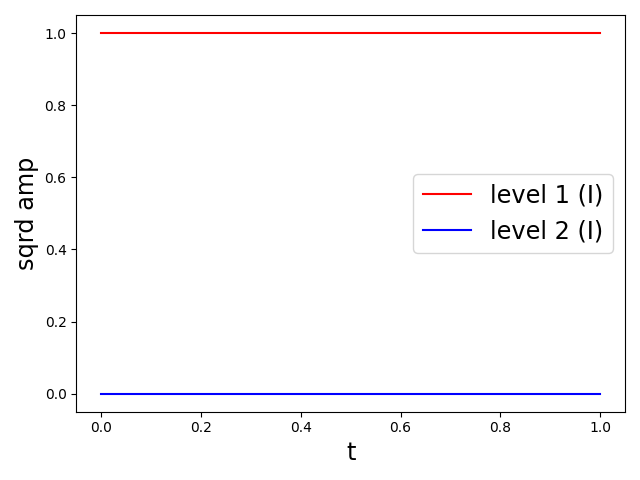
\includegraphics[scale=0.39]{542HW2/III_single.png}
\end{center}
\hfill\break
\hfill\break
\textbf{(a)} For initial state $|I\rangle = |2\rangle$ being the excited state, we plot $5$ realizations with $\Gamma = 5$. 
\begin{center}
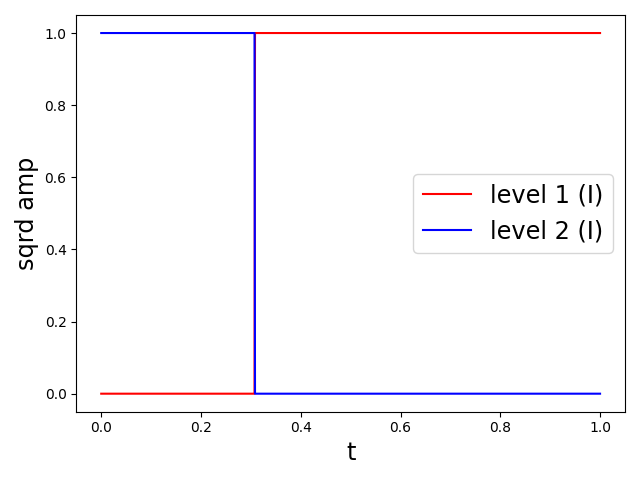
\includegraphics[scale=0.39]{542HW2/I/1I_single.png}\qquad
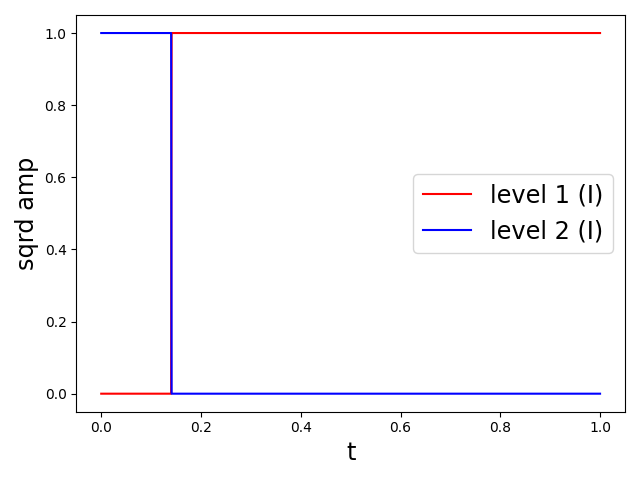
\includegraphics[scale=0.39]{542HW2/I/2I_single.png}\qquad
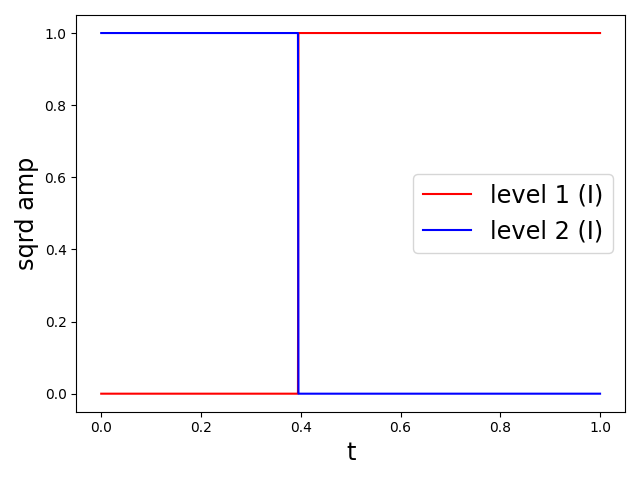
\includegraphics[scale=0.39]{542HW2/I/3I_single.png}\qquad
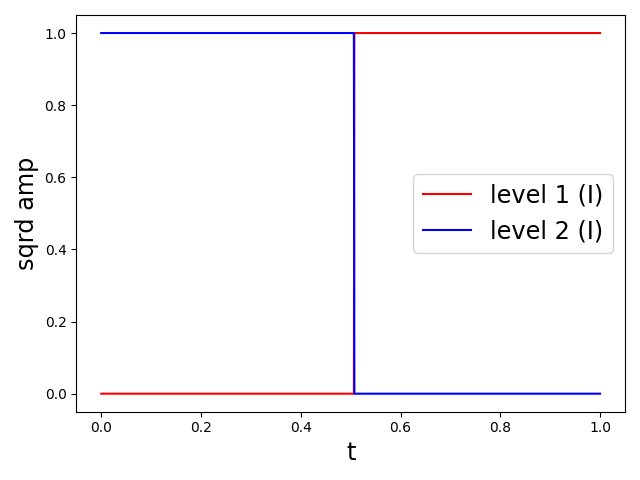
\includegraphics[scale=0.39]{542HW2/I/4I_single.png}\qquad
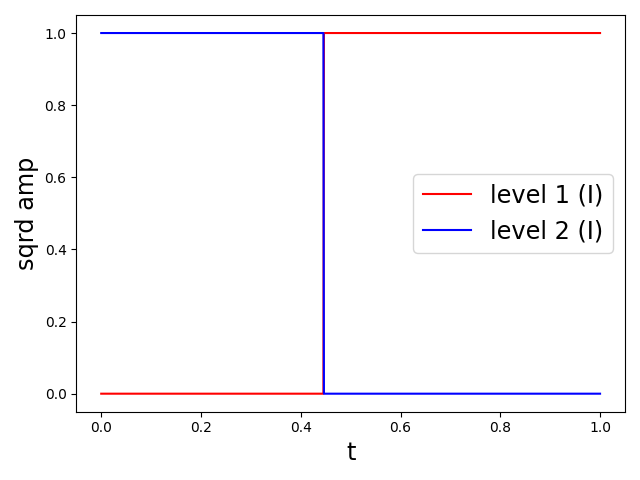
\includegraphics[scale=0.39]{542HW2/I/5I_single.png}
\end{center}

\newpage
\textbf{(a)} For initial state $|II\rangle = (|1\rangle+|2\rangle)/\sqrt{2}$, we plot $5$ realizations with $\Gamma = 5$. 
\begin{center}
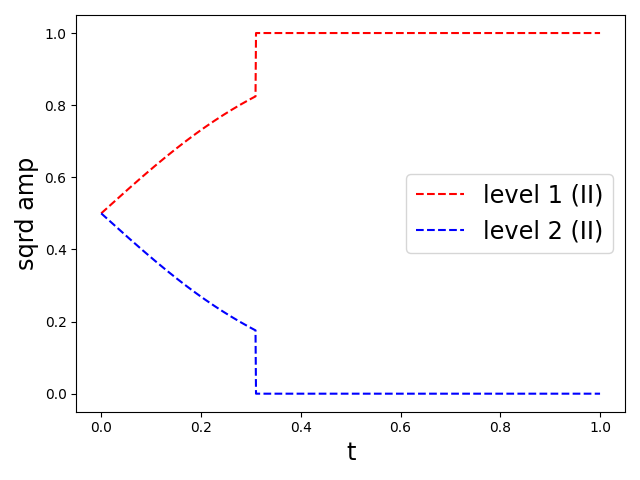
\includegraphics[scale=0.39]{542HW2/II/1II_single.png}\qquad
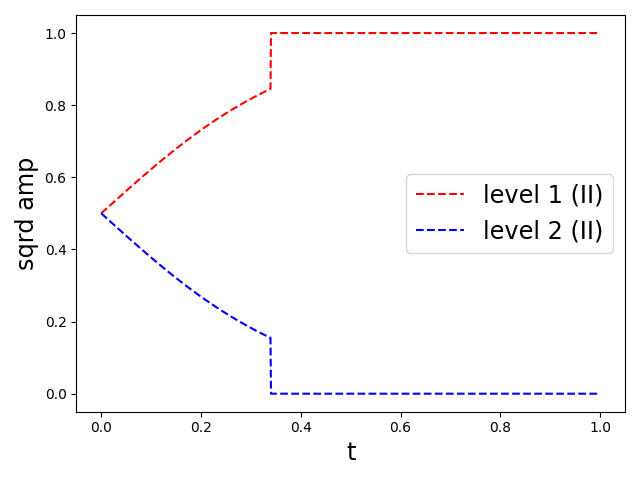
\includegraphics[scale=0.39]{542HW2/II/2II_single.png}\qquad
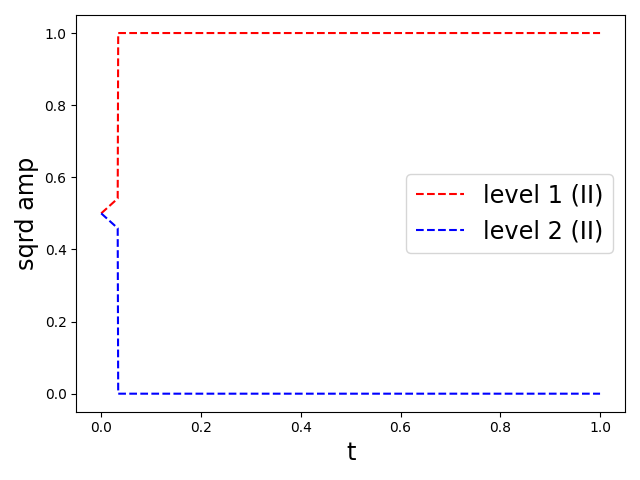
\includegraphics[scale=0.39]{542HW2/II/3II_single.png}\qquad
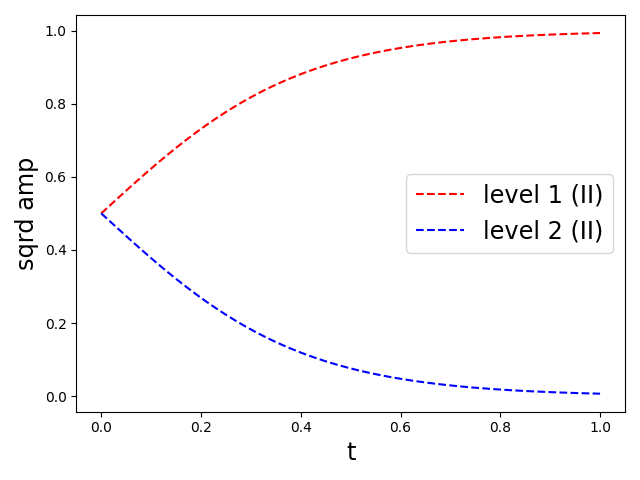
\includegraphics[scale=0.39]{542HW2/II/4II_single.png}\qquad
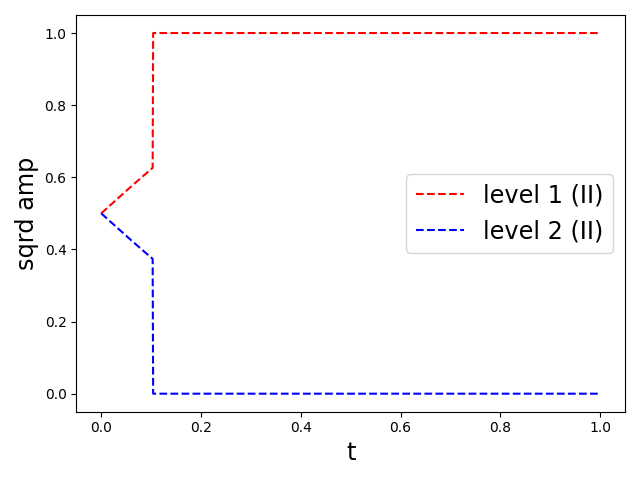
\includegraphics[scale=0.39]{542HW2/II/5II_single.png}
\end{center}

\hfill\break
\hfill\break
\textbf{(b)} For $|I\rangle$ and $|II\rangle$ averaged over $500$ realizations, we plot the squared amplitudes (in solid lines) comparing with the exponential decay curve (in gray dashed lines).
\begin{center}
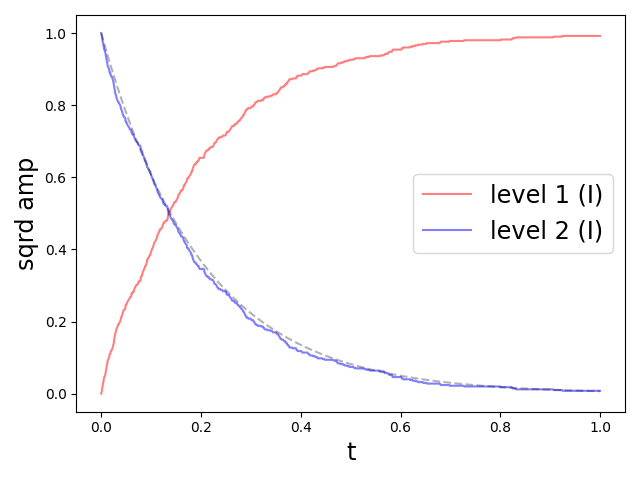
\includegraphics[scale=0.39]{542HW2/I_averaged}\qquad
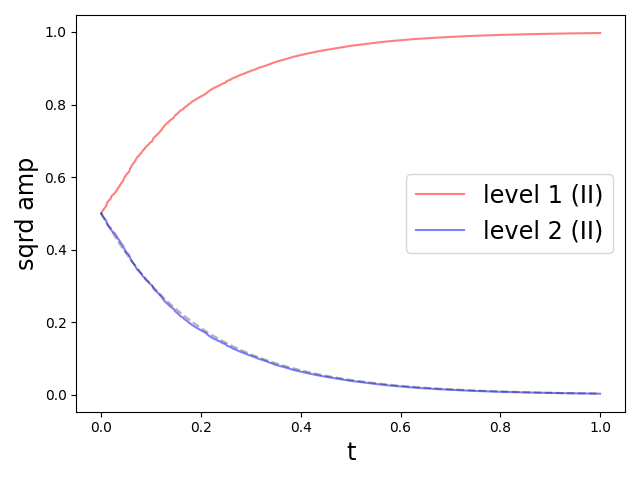
\includegraphics[scale=0.39]{542HW2/II_averaged}
\end{center}
We see here the solid curves (computed via MC method) follows closely with the dashed curves (exponential decay curve). 

\end{document}


